\documentclass[12pt]{article}

\usepackage[a4paper, total={7in, 9.5in}]{geometry}
\usepackage[english]{babel}
\usepackage{indentfirst}
\usepackage{fancyhdr}
\usepackage{setspace}
\usepackage{graphicx}
\usepackage{hyperref}
\usepackage{epsfig}
\usepackage{paralist}
\usepackage{lastpage}
% \usepackage[scaled]{helvet}
% \renewcommand\familydefault{\sfdefault}
\usepackage[T1]{fontenc}
\usepackage{url}
\usepackage{pgfplots}
\usepackage{tocbibind}
\usepackage{amsmath}
\usepackage{enumitem}
\usepackage{algorithm}

\pgfplotsset{compat=1.17}

\usepackage{xpatch}
\xpretocmd{\part}{\setcounter{section}{0}}{}{}

\pagestyle{fancy}
\fancyhf{}

\hypersetup{
  colorlinks=true,
  citecolor=blue,
  filecolor=black,
  linkcolor=blue,
  urlcolor=blue
}

\setlength{\parskip}{6pt}

\renewcommand{\headrulewidth}{0.3mm} % Top line width
\renewcommand{\footrulewidth}{0mm} % Bottom line width

\singlespacing

 \lhead{\hspace*{0mm}\raisebox{3mm}{
   \epsfig{file=~/Academia/TEX-Latex/logo/Aalto_en_1.pdf, height=11mm}}
 }

\chead{\hspace*{50mm}\raisebox{7mm}{\hspace*{60mm}\small\begin{tabular}{r}
      \textbf{Programing Studio 2}\\CS-C2120\\\today\\
\end{tabular}}}

%Footer
\lfoot{}
\cfoot{}
\rfoot{\thepage}

\newcommand{\argmax}{\operatorname*{argmax}}
\newcommand{\argmin}{\operatorname*{argmin}}

\begin{document}

\begin{titlepage}
    \thispagestyle{fancy}
    \begin{center}
        \vspace*{1cm}
            
        \huge
        \textbf{Documentation}
            
        \vspace{0.5cm}
        \Large
        Balancer\\

        \normalsize
        \vspace{0.5cm}
        Final Project for CS-C2120
            
        \vspace{1.5cm}
            
        \textbf{Hau Phan}

        \normalsize
        886690
            
        \vfill

            
        Bachelor Degree in Science\\
        Data Science Program\\
        Years of study: 2020-2023
            
        \vspace{0.8cm}
            
        \normalsize
        Department of Computer Science\\
        Aalto University\\
        Finland, \today
    \end{center}
\end{titlepage}
\newpage

\tableofcontents
\addtocontents{toc}{\protect\hypertarget{toc}{}}
\newpage

\section{General Description}
A strategy game where players tries to place weights on a set of scales while
keeping the scales balanced. The "riskier" the weight, the more score it yields.
Player with the most score win the round. The game spans over multiple rounds
and the winner is determined by the number of rounds won.
\subsection{Concepts}
\subsubsection{Weight}
A simple weight that have some mass. All the weights in the game have the same
mass of 1. The farther the weight from the scale center, the more score it
yields. Weights can be stacked.
\subsubsection{Scale}
A scale means a supported long "board" on which you can place other scales
and weights. Here the term "board" is used flexibly to mean the two arm of the
scale, the left arm and the right arm:
\begin{verbatim}

                               A
                           A   A       A     A
                          <1=A=1>   <3=2=1=?=1=2=3>
                             b             a
                             *           A *
                        <5=4=3=2=1=?=1=2=3=4=5>
                                   a
                                   *
               XXXXXXXXXXXXXXXXXXXXXXXXXXXXXXXXXXXXXXXXXXXXX
\end{verbatim}

The farther the weight from the center point, the more torque it applies to the
scale arm. The imbalance metric is the difference between the torques. Note that
a small imbalance is permissible. The maximum allowed magnitude of the imbalance
is the same as if 1 weight was placed at the end of the scale before the other
weights were set. That is, for a balanced scale, the total imbalance $\geq$ the
``radius” of the scale. (See examples below).  Once a scale is tipped/flipped,
it will be removed along with all its weights.

\newpage
\textbf{Example 1}
\begin{verbatim}

                   A
         A         A
        <3=2=1=A=1=2=3>
               a
               *
    XXXXXXXXXXXXXXXXXXXXXXXX
\end{verbatim}

If a weight is at a distance of 3 from the center of the arm, it pushes that
side down with the force of three weights. If the other side has two weights at
a distance of two, they push that side down with a force of four weights. (2 * 2
= 4). The imbalance is 3 - 4 = -1. The absolute value of the imbalance is less
than the radius of the scale, 3, so the scale is balanced.

\textbf{Example 2}

If the left arm of the previous example did not have a weight, the scale would
have been unbalanced (flipped) since the imbalance would have been 4, which
exceeds the radius of the scale. In this situation, the scale is flipped and all
the weights is lost.  

You can also place other scales on the scale. The scale placed on the second
scale applies a force equal to the sum of the weights and scales on it.

\textbf{Example 3}

\begin{verbatim}

             A
         A   A       A     A
        <1=A=1>   <3=2=1=?=1=2=3>
           b             b
           *           A *
      <5=4=3=2=1=?=1=2=3=4=5>
                 a
                 *
                 *
    XXXXXXXXXXXXXXXXXXXXXXXXXXXXXXXX
\end{verbatim}

Scale $b$ is balanced, the right-side weighs 2 * 1 and the left one 1 * 1 which
does not exceed the radius of the scale. The scale B itself weighs three
weights.

Scale $c$ is balanced since the left side weighs 1 * 2 = 2 and the right side 1
* 1 = 1. The difference of these is 1, which does not exceed the radius of the
balance. Scale $c$ weighs 2 weights!

Scale $a$ is also balanced. On the left side there is a scale $b$ at a distance
of 3, 3 * 3 = 9. On the right there is scale $c$ at a distance of 4, 2 * 4 = 8,
and a weight at a distance 3. All together there is a weight of 11 weights on
the right side. The difference is 11 - 9 = 2, which is smaller than the radius
of scale $a$, so the scale is balanced.

\subsubsection{Players}
There are two type of players: \textbf{human} and \textbf{bot}. Multiple players
(recommended 2-3) can play the game at any one moment.
\subsubsection{Capture and ownership}
\label{sec:cap}

Both the \textbf{weights} and \textbf{scales} during each round is either
\textbf{player-owned} or \textbf{wild} i.e owned by no one. The wild weights and
scales are placed randomly at the beginning of each round and can be captured by
players. Players can also captures each other weights and scales. Captured
scales give addition "buffs" for the owner's weights while capture
weight give points. Initially, the weight is owned by the player making the
move.

Weights can be \textbf{stacked}. One can capture all the weights underneath by
placing his/her weights on top. To capture a scale, one must have \textbf{at
least} $r$ more weights than the player with the 2nd most weights, where $r$ is
the radius of the scale. (See examples below)

Owner of a scale will have the following benefits:
\begin{itemize}
  \item His/her weights on the scale can not be captured, even when other
    players place the weight on top. The moment the scales' owner change, all
    weight that should be captured will be updated according to the rules.
  \item Each of his/her weight will have its score multiplied by 2.
\end{itemize}

\textbf{Example:}
\begin{verbatim}
                   A
             A B   A C
            <2=1=A=1=2>
                 a     
                 *     
                 *    
       XXXXXXXXXXXXXXXXXXXXX
\end{verbatim}

Here the scale is captured by player A, since there are 3 A weights and only 1 B
and C weight. The difference is $3 - 1 = 2 \geq 2$ the radius of the scale. The
letter A at the middle indicates the owner of the scale


\subsection{Rules and Gameplay} 
\subsubsection{Gameplay}
\begin{itemize}
  \item There is a predefined number of round in one game. (Usually 5 for 2-3
    players)
  \item Each round will have a fixed number of weights that all players will
    draw from and place onto the scales. (Usually 10-15 weights per round)
  \item At the beginning of each round, one scale and 5 wild weights will be
    randomly placed by the computer with some predefined probability.
  \item The round starts and the players place the weights one at a time on the
    scales. 
  \item The round is over when there is no weight left. The scores are then
    calculated and the player with the highest score win the round.
  \item The next round then starts and \textbf{continues} from the last round's
    state.
  \item The player who win the most round wins the game.
\end{itemize}
\subsubsection{Scoring}

\textbf{Example:} 
\begin{verbatim}

            A
      A B   A
     <2=1=A=1=2>
          b          
          *         C B
          *   ?     C B
         <3=2=1=?=1=2=3>
                a
                *
                *
    XXXXXXXXXXXXXXXXXXXXXXXXXXXXXX
    Status: equalibrium 

    a: scale b: (2 * 1 + 1 * 2) * 2 = 8 points 
       scale a: 3 * 8 = 24 points
       -------------------------------
       total: 24 points

    b: scale b: 1 * 1 = 1 points
       scale a: 3 * 1 + 3 * 2 = 9 points
       -------------------------------
       total: 9 points

    c: scale a: 2 * 2 = 4 points
       -------------------------------
       total: 4 points
\end{verbatim}

Here '$?$' represents wild weights and uncaptured scales. 

The scale with index 2 is capture by the player "a" so its points is multiplied
by 2

\subsection{Difficulty level}
Completed level of difficulty: Intermediate/Difficult

The project succeed in meeting all the requirement of Easy and Intermediate
criterions. Both a console-based and graphical user interface was implemented.
To meet the Difficult requirements, an intelligent computer opponents was
implemented along with additional game mechanics such as capturing scales, 
weights and random computer-generated scales. The project also aim at a creating
a fully functional game: splash art, animations and tile textures is also added
to improve the visual of the game.



\section{User interface}

\subsection{Graphical}


\subsubsection{Game loop}

When the user open the game, a splash screen is shown with animated logo and
background. The user can click on the top left of the menu bar to select a new
game, load a saved game or quit.

If the user choose to start a game, the game then switch to the game screen where player can interact with the game. 

The game screen is shown on the left side of the window. Player can click
directly on the scale to place the weight, dragging to pan screen and scrolling
to zoom in and out.

The game information is shown on the right side of the window. This includes the
score of each player, the number of rounds won by each player, the round number,
how many weights left in the pool, \dots. There are also undo and redo buttons
to undo previous moves, and buttons to add additional scales and weights if
needed.


At the end of the round, a pop-up will be shown and announce the round's winner.
The game then continues to the next round, randomly placing 5 weights and a
scale. If it is the final ground, a pop-up will announce the game's winner
instead.

\begin{figure}
  \centering
  \caption{The splash screen}
  \includegraphics[width=\textwidth]{graphic1.png}
  \label{fig:gra1}
\end{figure}
\begin{figure}
  \centering
  \caption{The game screen}
  \includegraphics[width=\textwidth]{graphic2.png}
  \label{fig:gra2}
\end{figure}
\subsubsection{Actions}

Player can choose to start a new game by clicking "File" > "New" or go back to
the menu with "File" > "Back to Menu".

At any moment, the user can choose to save the game by clicking "File" > "Save",
exit the game completely by "File" > "Exit" or go back to the splash screen by choosing "File" >
"Back to Menu"

\subsubsection{Settings/Options}

Additional players can be added by clicking the "Edit" > "Add Human" and "Edit"
> "Add Bot". Undo and Redo button can also be found in the "Edit" menu.

The rules and additional informations on the game can be accessed via the "Help"
menu in the menu bar.


The source code is also available by clicking the "Help" > "Github" and "Help" >
"Gitlab", which will open the repository using the default browser.

\subsection{Console-based}
The program can be run on the command line with no arguments to start a new game
or path to the save file to resume. A sample game are shown below:


\begin{verbatim}
============ ROUND  1 ============
_________________________________________
| Ben   (B, 0) :    56 points (human)   |
| Ken   (K, 0) :   248 points (  bot)   |
| Jaiden (J, 0) :    63 points (  bot)  |
|_______________________________________|




       <5=4=3=2=1=?=1=2=3=4=5>
                  g
                  *
            J K   *   K K
           <4=3=2=1=?=1=2=3=4>
                    e
              ?     *
              B J   *       ?
             <2=1=?=1=2>   <1=?=1>
                  d           f
      K           *           *
      K           *           *
      K K         *           *
      K K         *         ? *     B
      K K     J ? *         K *   ? B
     <3=2=1=K=1=2=3>       <2=1=?=1=2>
            c                   b
            *       ? J   B     *
    ?   ?   *   B   B J   B J J *
   <7=6=5=4=3=2=1=?=1=2=3=4=5=6=7>
                  a
                  *
XXXXXXXXXXXXXXXXXX*XXXXXXXXXXXXXXXXXXXXXX
>>>>>>>>> BEN   TURN <<<<<<<<<
Which scale ? (d,b,g,e,f,c,a): a
Position ? [-7,7]: 1
\end{verbatim}


\subsubsection{New Game}

When a new game starts, the game will prompt the user to enter basic information
about the players. The first round then starts and each player will in turn be
prompted for information on where his/her weight should be placed. The current
scoreboard, the state of the game will also be shown to for players to make
their decision.

When a round finished, the winner of that round will be announced. At the end of
the game, the final winner will be announced instead.

\subsubsection{Load Game}

When the save file is loaded successfully, the game will continue from the state
when it is saved. If an error occurred, the line causing the
failure will be printed.

\section{Program Structure}

\begin{figure}
  \centering
  \caption{The balancer package structure}
  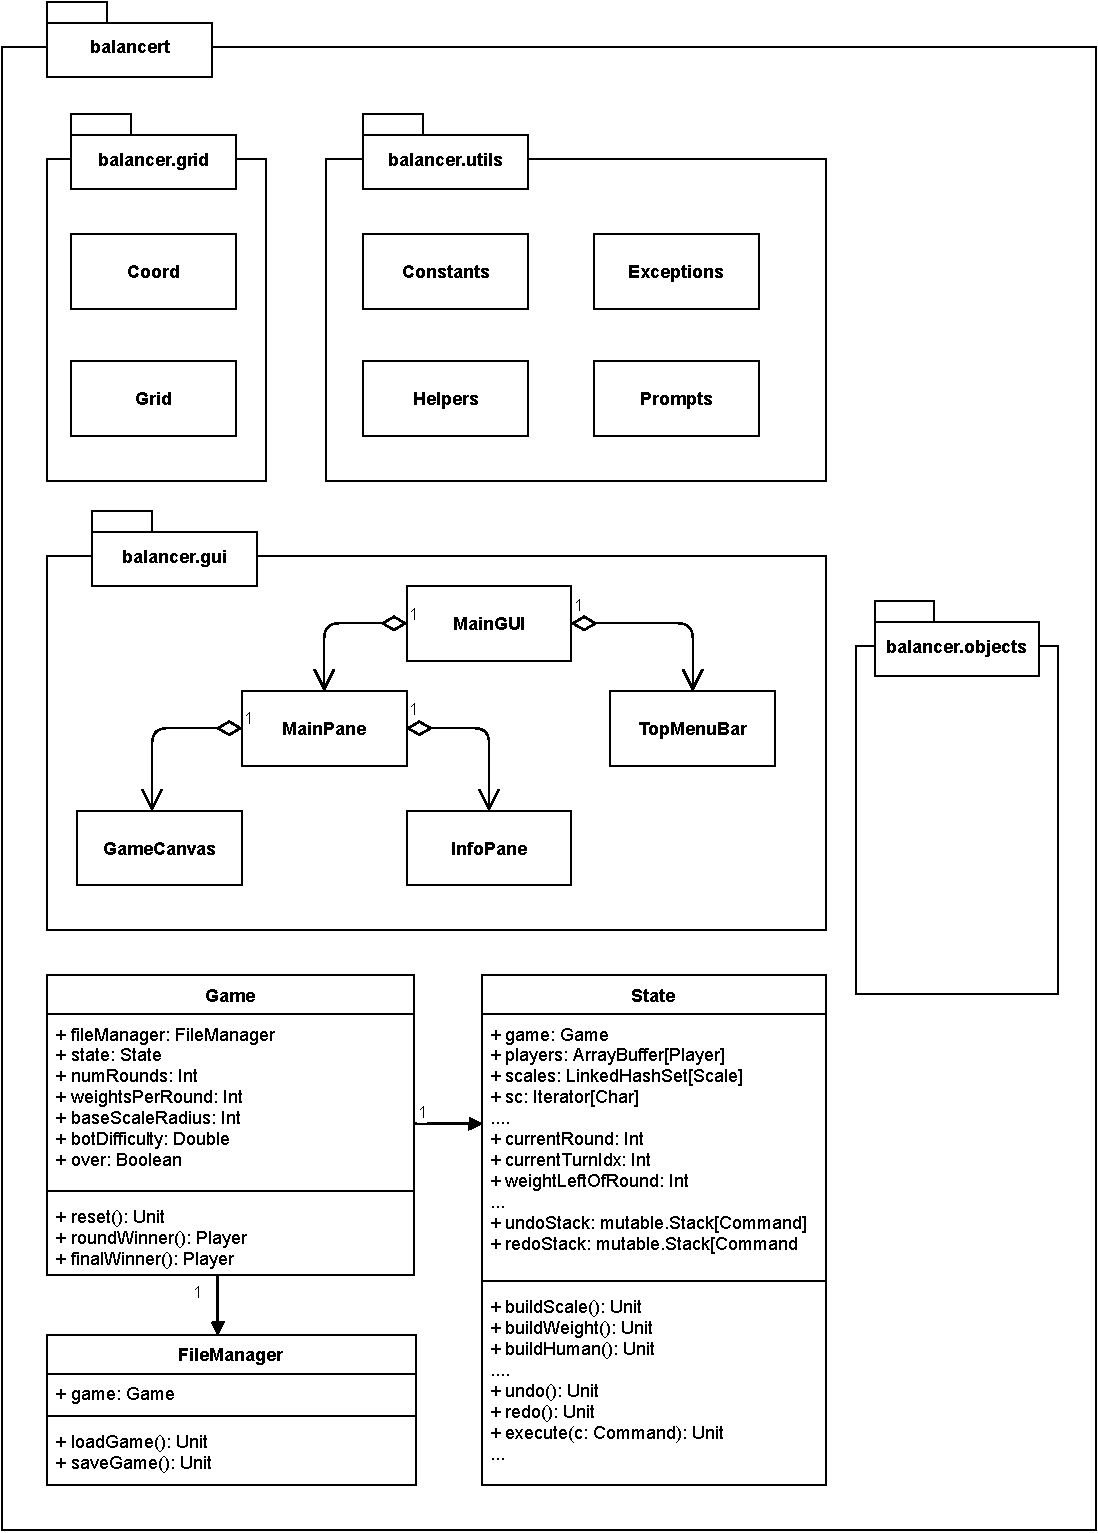
\includegraphics[width=\textwidth]{UML1.pdf}
  \label{fig:uml1}
\end{figure}

\begin{figure}
  \centering
  \caption{balancer.objects UML}
  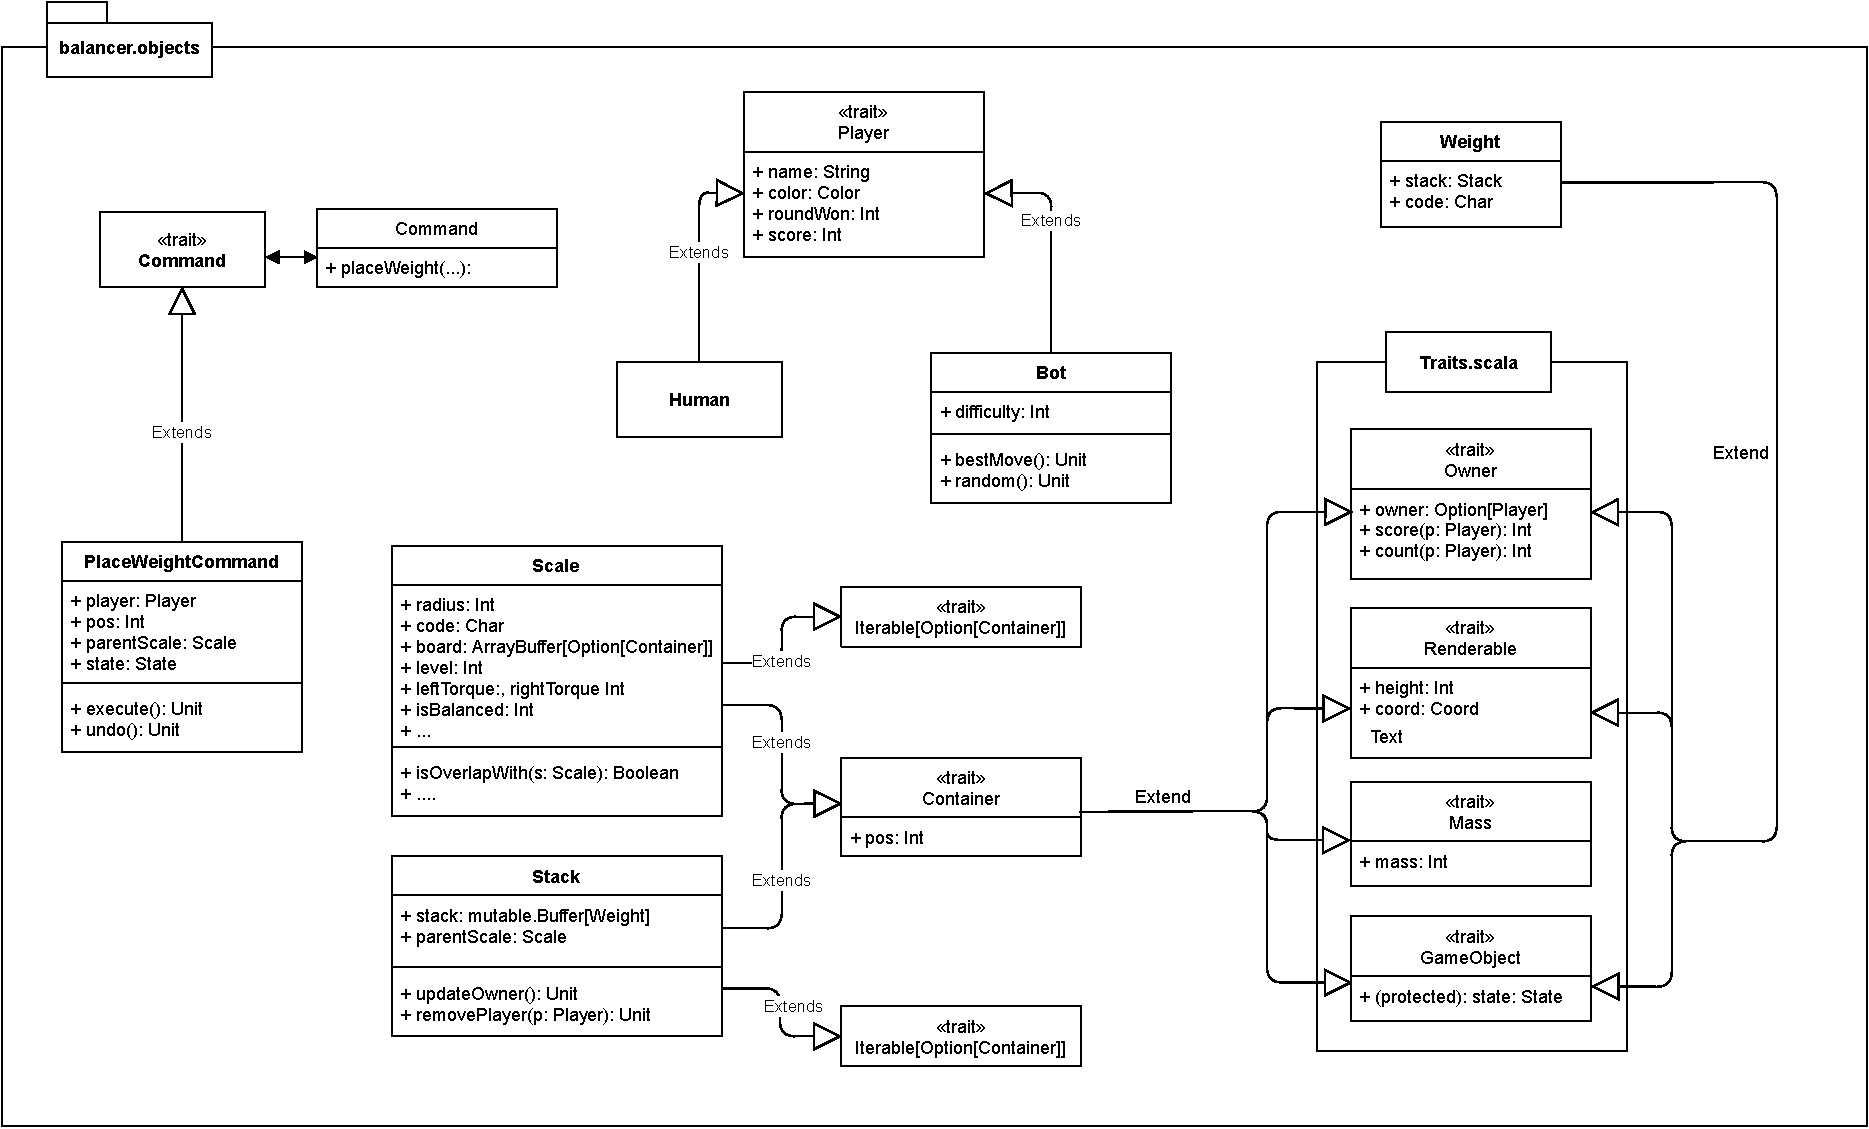
\includegraphics[width=\textwidth]{UML2.pdf}
  \label{fig:uml2}
\end{figure}

The program is split into packages, categorized according to their
functionalities and roles in the program. The top most package is
\textit{balancer}, containing the class \textbf{Game}, \textbf{FileManager} and
\textbf{State}. \textbf{Game} stores basic default settings of the game such as
the number of weights per round and the default difficulty of the bot. It also
acts as a mounting point for \textbf{State}, which is different for each game
and thus, change whenever the user save or load.  \textbf{FileManager} handles
all operations regarding saving and loading \textbf{State}. \textbf{State}
models the game's state, which is any relevant information that changes during
the game, and thus unique for each game. The other subpackages of
\textit{balancer} include:

\begin{itemize}
  \item \textit{balancer.grid:} contains the class \textbf{Grid} and
    \textbf{Coord}. \textbf{Grid} model a grid of character, an abstract
    representation of the game state. Each character can either represent a
    weight of a player, a part of the scale or an empty space. In other terms,
    grid are just a collection of tiles to display the game.The \textbf{Coord}
    class models a simple 2D coordinate or point, with basic arithmetic such as
    adding and subtracting.
  \item \textit{balancer.utils} contains the objects \textbf{Constants, Helpers,
    Prompts} and \textbf{Exceptions}. \textbf{Constants} and \textbf{Helpers}
    are quite self-explanatory, they store different constants and helper
    functions. \textbf{Prompts} stores wrappers of the default scalafx's
    \textit{Alert} class. They ranges from informing the users, asking for user
    inputs and open the file-chooser dialog to save the game.
  \item \textit{balancer.gui} contains wrappers of scalafx's components and
    \textbf{MainGUI}, which is the entry point of the application.
    \textbf{MainPane} is a wrapper class of scalafx's SplitPane, modeling the
    main area of the game. \textbf{TopMenuBar} extends the scalafx's MenuBar,
    modeling the app's menu bar, while \textbf{GameCanvas} extends the default
    scalafx's ScrollPane, allowing for panning and zooming. A canvas is also
    attached and used to display the game's grid. \textbf{InfoPane} is the left
    pane that is in charge of display other relevant stats/information of the
    game, such as the score of each player and the number of weights left in the
    round.

  \item \textit{balacner.objects} contains objects that model different aspect
    of the game's mechanics. The relationships between them are shown in Figure
    \ref{fig:uml2}. \textbf{Command} models a command or a move from a player.
    Here, there is only one the place weight command is implemented.
    \textbf{Scale} and \textbf{Stack} models the in-game scale and stack of
    weights. \textbf{Traits.scala} stores share traits between \textbf{Scale},
    \textbf{Stack} and \textbf{Weight}. \textbf{Stack} and \textbf{Scale} also
    implements the methods of the \textbf{Iterable} trait, allowing to be looped
    over and its content accessed by index, similar to scala's \textbf{Seq}.
    \textbf{Player} models a generic player, with a unique name, color and basic
    stats such as the number of round won and score. \textbf{Human} and
    \textbf{Bot} extend from \textbf{Player}, modeling a human player and a bot
    player respectively.

    % // NOTE TO SELF: FIX THE UML MODEL
\end{itemize}

\section{Algorithms}
\subsection{Attributes}
Due to the recursive nature of the game (scale on scale on scale), most methods
and attributes are either call other recursive methods or recursively defined
themselves:
\begin{itemize}
  \item scale's \textit{mass} = the sum of its stack's \textit{mass}
  \item stack's \textit{mass} = the sum of its weight's \textit{mass}
  \item scale's \textit{level} = the parentScale's height +
    1 (0 if at the bottom)
  \item \textit{imbalance}: 
    \begin{align*}
      \text{Imbalance} = \sum_{i=-r}^{r}i\;m_i
    \end{align*}
    where $r$ is the radius of the scale, $m_i$ is the mass of the object at
    distance $|i|$ from the center. Negative value of $i$ indicates the object
    is on the left arm of the scale.
  \item \textit{score}: player $p$'s \textit{score} on an object $o$ is a
    piecewise function conditioned on $o$ and $p$:
    \begin{equation*}
      s(o,p) = \begin{cases}
        s(o, p) = \sum_{i=-r}^{r} |i|\;s(o_i, p) , &\text{ if $o$ is a scale}\\
        s(o, p) = \sum_{w\in S} s(w, p) , &\text{ if $o$ is a stack, with
        weights $S$}\\
        s(o, p) = 1 &\text{ if $o$ is a weight owned by $p$}\\
        s(o, p) = 0 &\text{ if $o$ is a weight not owned by $p$}
      \end{cases}
    \end{equation*}
    where $o_i$ is the object at distance $|i|$ from the center the scale.
    Negative $i$ indicates the object is on the left arm.
\end{itemize}
\subsection{Intelligent bot}
\subsubsection{Description}
\begin{itemize}
  \item \textbf{randomized:} The randomized bot simply searches for all moves
    and filters out moves that would tip a scale, then randomly pick a move.
  \item \textbf{semi-greedy:} The semi-greedy bot also searches for all moves
    and filters out moves that would tip a scale, but then pick the move that
    yields the most point for the bot instead.
  \item \textbf{mixed:} a random number generator is used to determine which
    algorithm to use among the above twos.
\end{itemize}
The \textbf{randomized} bot can check if a move will result in any scale flipped
by "faking" the move: place the weight, recursively check if any scale is
flipped then revert the move. Similarly, the \textbf{semi-greedy} bot can
implement a similar method and calculate the score before reverting back, thus
finding the move that yield the highest score.

Computing time is nearly instant for most game with only human players, which
should be at most 5-6 scales per round. 

\subsubsection{Limitations}
Since the bot will never tip a scale, human players can exploit this
characteristic of the bot to their advantages and flip a scale deliberately to
come out on top. A true greedy bot will also takes moves that will tip a scale
into consideration.

\subsection{Randomized Generation}

\textbf{Avoiding collision when generate scale}: 
A simple brute force algorithm is implemented to place random scale without them
overlapping each other: finding all possible empty positions, randomly pick a
position, "fake" placing the scale and check if collide with any scale of the
same level, if it is, revert the placement.

\textbf{Weight generation:} 
A similar algorithm to the \textbf{random-bot} algorithm is used: Search for
all possible moves that wouldn't tip any scale if played, then randomly execute
one of those move.

\section{Data Structures}

\textbf{Grid} is implemented as a 2D \textbf{Array} of character (\textbf{Char})
due to it performance (constant access and insertion time). Since \textbf{Grid}
will be modified frequently (whenever there is a change in the game state),
quick access, insertion and initialization is crucial for performance. Since
most of the grid entries are empty, the grid is \textit{sparse}, and some
optimization can be done. Other data structures such as HashMap and R-Tree was
also considered for more efficient memory usage of sparse matrix, however since
the dimension of our grid is not too large ($< 10000$), the memory
saved/performance trade offs due to overheads might not be desirable.
Implementing a grid as a 2D \textbf{Array} also help in development due to its
familiarity.

\textbf{State} also contains a cached collection of references to the scales,
since traversing the scale recursively might not be efficient for some
operations. The scales collection is implemented as scala mutable collection
\textbf{LinkedHashSet}, since we need a mutable collection of unique elements
with constant access time and good insertion time. \textbf{LinkedHashSet} is
only used during development, however, since the elements are ordered (scale
inserted first will be accessed first), which will help during debugging and
testing. During deployment, the default \textbf{HashSet} will be used instead to
reduce overheads (linking). The program is designed to better handle large
amount of scales. However, it is known that the average number of scales might
not exceed $10$ in most game with human players, thus \textbf{ArrayBuffer} might
be a better alternative. \textbf{State} will also stores a collection of
\textbf{Player} which be implemented as scala's \textbf{ArrayBuffer}.

\textbf{Stack} is implemented as a \textbf{Buffer}, since it provides much of
the functionality of a stack and easy to work with.  The \textit{board} of
\textbf{Scale} will be modeled as a immutable \textbf{Array} since its length is
constant i.e the scale can not shrink or grow in length. Raw access speed and
low overhead is also one reason to choose the default \textbf{Array} over
\textbf{Buffer} for \textit{board}.


\section{File and Internet Access}

The state of the game is saved in a semi-human-readable format:

\begin{verbatim}
    BALANCER 1.0 SAVE FILE
    # Setting
    WeightPerRound: 15
    NumberOfRound: 5
    BotDifficulty: 0.5
    # Meta
    Human: Ben
    Bot: Ken,Jaiden
    Round: 1
    Turn: Ben
    # Scale
    _,0,7,a : -5,? | -1,B | 1,B | 2,J,J | 4,B,B | 5,J | 6,J
    a,7,2,b : -2,K | 2,B,B
    a,-3,3,c : -3,K,K,K,K,K | -2,K,K,K | 1,J | 2,?
    c,3,2,d : -2,B | -1,J
    d,1,4,e : -4,J | -3,K | 1,K | 2,K
    b,-1,1,f : -1,?
    END
\end{verbatim}

\begin{itemize}
  \item The first line of the file is of the form: 
    \begin{align*}
      \text{BALANCER (VERSION) SAVE FILE}
    \end{align*}
  \item The file is split into blocks. Each block of data has a header and a
    body. A header is identified by having "\#" prepended. The header marks the
    start of a block.
  \item Each row in the body contains information about the game and is of the
    form:
    \begin{align*}
      \text{IDENTIFIER : DATA}
    \end{align*}
    \item The IDENTIFIER and DATA is different for different blocks.  There are
      3 types of block: \textit{Setting, Meta} and \textit{Scale}.
  \item The \textit{Setting} block contains different configurations of the saved game.
  \item The \textit{Meta} block contains metadata of the saved game. 
  \item The \textit{Scale} block contains the position of each scales and weights when
    the game is saved. The IDENTIFIER is the scale's position and the DATA is
    the position of each weight on the scale:
  \item For example, this line in the \textit{Scale}  block:
    \begin{verbatim}
                        a,7,2,b : -2,K | 2,B,B
    \end{verbatim}
    from left to right indicates: the parent scale code ("a"), the position on
    the parent scale (on the right arm, distance 7 from the center) and the
    radius ($=2$) \item After the colon are the weights' position on the scale,
    it must be listed from left to right (thus the indices must be from smallest
    to biggest). 
    \begin{itemize}
      \item (-2,K) indicates on the left arm, distance 2 from the center, there
        is a weight belong to Ken (K).
      \item (2,B,B) indicates on the right arm, distance 2 from the center,
        there are 2 weights stacked on each other, both belong to Ben (B). The
        bottom weight is on the right.
    \end{itemize}
  \item The END keyword represents the end of the saved file. Any line after
    this keyword is not interpreted by the parser.
  \item \textit{Note: for the bottom most scale, the parent scale code is "\_",
    and the position is $0$. "?" indicates this is a wild weight or scale, i.e,
  with no owner. Any excess white space will be ignored by the parser.} 
\end{itemize}

\section{Testing}

The program is tested manually by typing onto the console (for text-only
version) or interacting with the graphical UI directly (in a graphical window).
These tests include:
\begin{itemize}
  \item The weight is placed at the correct position according to the user mouse
    position.
  \item Panning and zooming work correctly.
  \item Information/Status of the game such as the score, the round number and
    the number of weights are displayed correctly.
  \item \textbf{GameCanvas} accurately displays the current state of the game
    and update when a new weight is placed.
\end{itemize}

There are automated tools to system test graphical user interfaces. However,
running the game directly is the most straightforward one. Different save files
are created and purposely designed to test different aspects of the game,
specifically, accurate balance-checking of the scales, bot algorithms and random
weight, scale generation. 

Important "core" methods and attributes that are used frequently through out the
program are unit-tested. Example of these "core" methods are the
\textit{buildWeight()} and \textit{buildScale()} of \textbf{State}. They have
multiple test cases designed specifically to test there accuracy. Some tests
also aim to test how "solid" these methods are by presenting edge cases and
invalid inputs.

Beside "core" methods, algorithms is also tested frequently for accuracy, i.e
they do what they are supposed to do. The two algorithms that will be tested
extensively is the \textbf{semi-greedy} bot's algorithm and the rendering
algorithm for update the game's grid. 

Only some methods and algorithms passed the tests during their first
implementation. Most of them failed and reveal many obscure bugs and faulty
logic in the code. The semi-greedy bot algorithm is most tested and also failed
the most. Testing really helped speeding the debugging process.

The loading and saving of game file is also tested intensively. There might
still be bugs in the implementation since there are a lot of edge cases for
human-readable/modifiable save file.

\section{Known bugs and missing features}

\subsection{Bugs and Temporary Fixes}

A possible area where bugs can occur is during the loading and saving of the
game. The custom parsing function \textit{loadGame()} is done rather "hacky" and
unidiomatic, which may contains obscure bugs that hard to identify. However, a
general try-catch safeguard is implemented to at least catch these errors and
notify the users.

Another possible bug that might occur is when there are players with similar
first letter name (e.g Jack and Jason, Mike and Mary\dots). Since the
\textit{weightCode} is the first letter of the its owner's name, their weights
will be represented by the same \textbf{Char} on the grid and considered as
belong to the same player. This is likely to cause many weird behaviors in the
game. Thus, to prevent this, the game will throw an error and notify the player
if such naming collision happen.

There are also extreme game state that can be achieve if users want to purposely
breaking the game, such as adding infinite number of scales or players. There is
a max-depth limit for recursion in Java/Scala, thus, exceeding this limit will
cause the program to throw an error when executing/calculating any recursive
methods/attributes. The number of scales might also exceed the ASCII limit for
lowercase letter ($z = 122$) and thus, assign weird characters to new scales.
However, both of these problem can be fixed by limiting the number of scales to
$26$.

On the opposite end, the game might also have $0$ player or only consists of
bots. This is also likely to cause an error and thus, at least one human player
are required for the game to start.

\subsection{Missing Features}

\textit{Multiplayer supports:} The original plan includes implementing a basic
multiplayer version of the game using \textit{Play framework}'s Websocket.
However, due to the time constraint, overlapping schedules and heavy workload
from other courses, it was not realized.

\textit{Setting Menu:} It was also planned, in the first version of the
technical plan, to implement a setting menu, which would allow users to modify
the settings directly in the GUI. However, it has not been implemented in time
of submission.

\textit{Full Undo:} Undoing is not fully implemented for scale. When a scale is
flipped, no undoing can be made to reinstate that scale.

\section{Best sides and Weaknesses}

\subsection{Best sides}
\begin{enumerate}
  \item The program is quite organized and can be easily to expanded/build upon
    in the future. Each packages is separated according to its roles in the
    program: \textbf{Helpers} contains helper functions and \textbf{Constants}
    stores different constants that are used. GUI elements are separated and
    explicitly named after their roles: \textbf{TopMenuBar}, \textbf{MainPane},
    \textbf{GameCanvas}, \dots 
  \item Undoing and Redoing are not planned in the original plan but are a
    result of refactoring to the class \textbf{Command}. While there are only
    one command (\textbf{PlaceWeightCommand}) for now, other commands such as
    \textbf{AddingPlayer}, \textbf{RemovePlayer} , \textbf{AddScale} ,
    \textbf{RemoveScale} \dots can easily be added using the same framework.
\end{enumerate}




The program can be divided into different areas/sections, grouped by its
role/concept that needed to be built, tested and documented. Here we also
introduce the concept of \textbf{"core"} classes and objects, parts of the
program that many other objects depend on them. In this project, they are the
main Game class, Weigh-Scale-Stack classes and the Player class. These
represents the fundamental ideas of the game and with them, gameplay is
achieved. Other classes will be build on top of them to either adding additional
functionality like save/load file or display them to the user either in a
graphical UI or on the console.

Different areas/sections will require different amount of time to go through the
3 phase mentioned above (built, test, document), with the core classes and the
UI being the most demanding ones. 

\begin{itemize}
  \item  The first two weeks (\textbf{22.2} - 7.3) will be dedicated to build
    and test different functionalities of these core classes. The bot algorithm
    may or may not be implemented in this period since it is not immediately
    essential and can be separated.
  \item The week after (8.3 - 14.3) will be dedicated to implement and test the
    save/load file functionality of the game. This will be important for testing
    the UI and the bot algorithm since generating test case will be much easier.
    Noted that the first interim report is due on 17.3.
  \item  The next 2.5 weeks (15.3 - 31.3) will be dedicated to build and test
    the UI for the game, on the console and graphically in a window. Noted: the
    second interim report is due on 31.3.
  \item  The next two weeks (1.4 -  14.4) will be dedicated to system testing of
    the whole program, debugging, tuning, optimizing for performance and adding
    additional features where needed. The final interim report is also due at
    the end of this period, on 14.4.
  \item  The final two weeks (14.4 - \textbf{28.4}) will be dedicated to writing
    the required documentation and act as a "buffer zone" if more time is needed
    to complete certain features.
\end{itemize}

\nocite{nystrom2014game}
\nocite{scalacollection}
\bibliographystyle{unsrt}
\bibliography{/home/phanth/Academia/TEX-Latex/bib.bib}
\end{document}
